%%%%%%%%%%%%%%%%%%%%%%%%%%%%%%%%%%%%%%%%%%%%%%%%%%%%%%%%%%%%%%%%%%%%%%%%%%%%%%
% CONTRIBUTION TO THE MESONH BOOK1: "Microphysical Scheme for Warm Clouds"
% Author : Evelyne Richard
% Original : October 15, 1997
% Update   : October 15, 1997
%%%%%%%%%%%%%%%%%%%%%%%%%%%%%%%%%%%%%%%%%%%%%%%%%%%%%%%%%%%%%%%%%%%%%%%%%%%%%%%

\chapter{Microphysical Schemes for Warm Clouds}
\minitoc
Three microphysical schemes for warm clouds are implemented into Meso-NH.
The most simple scheme is the Kessler one, a one-moment scheme that prognoses mixing ratio of cloud and rain water.
The two others are some two-moment schemes that predicts the mixing ratio and the concentrations of cloud and rain drops.
The C2R2 scheme is the most general one while the KHKO scheme is designed for stratocumulus.

\section{Kessler scheme}

%{\em by E. Richard}

\subsection{Equations}
We note $r_v$, $r_c$, and $r_r$ the water vapor, cloud water and rainwater
mixing ratios, as defined in MESO-NH. For any constituent,
$r$ is the mass of the
constituent divided by the reference mass of dry air.\footnote{Notice that
$\rho_{d\, ref}r = \rho_d \tilde r$ where  $\tilde r$ is the usual mixing ratio
i.e. the mass of the constituent divided by the mass of dry air.}
The consevation equations for these quantities are written:
\begin{eqnarray}
 &\dfrac{d}{dt}(  \rho_{d\,ref} r_v)&= \rho_{d\,ref} (P_{RE}-  P_{CON})\\
 &\dfrac{d}{dt}(  \rho_{d\,ref} r_c)&= \rho_{d\,ref}(- P_{RA} -  P_{RC}+  P_{CON})\\
 &\dfrac{d}{dt}(  \rho_{d\,ref} r_r)&= \rho_{d\,ref} (P_{RA} +  P_{RC} -  P_{RE}
+  P_{RS})
\end{eqnarray}
where $P$ designates the sources and where the subscripts
 $CON$, $RE$, $RA$, $RC$ and $RS$  respectively refer to the following processes:
evaporation/condensation, rain evaporation, accretion of cloud droplets by
raindrops, conversion of cloud droplets into raindrops (autoconversion),
and rain sedimentation.
Condensation/evaporation is a very fast process, it cannot be computed
explicitly and is obtained through an implicit saturation adjustment
procedure, taking subgrid-scale processes into account (see Chapter on the sub-grid condensation schemes).
All others terms are computed explicitly.


\subsection{Raindrops characteristics}
\subsubsection{Distribution}
Raindrops are assumed to follow a Marshall-Palmer distribution. The number of
raindrops whose diameter lies in the interval
$D$ and $D+dD$ is given by:
\begin{equation}
N(D)dD=N_0 \exp (-\lambda D) dD
\end{equation}
Observations for different types of rain show a range of values for
$N_0$ from
$0.4\ 10^7$ to $3.5\ 10^7$~m$^{-4}$. $N_0= 10^7$~m$^{-4}$
is a value frequently used.


The $\lambda$ parameter is obtained from
\begin{equation}
 \rho_{d\,ref} r_r=\int_0^\infty {\pi \over 6} \rho_{lw} D^3 N_0 \exp(-\lambda D)dD=
{\pi \rho_{lw} N_0 \over \lambda^4},
\end{equation}
which leads to
\begin{equation}
\lambda= \Big({\pi \rho_{lw} N_0 \over \rho_{d\,ref} r_r}\Big)^{1 \over 4}.
\end{equation}
\subsubsection{Fall velocity}
The terminal fall velocity for a raindrop of diameter $D$ is expressed as
\begin{equation}
V(D)=  \big( \dfrac{ \rho_{00}}{ \rho_{d\,ref}} \big)^{\alpha} aD ^{b},
\label{eqvterm}
\end{equation}
with $\alpha=0.4$, $a=842$~m$^{0.2}$/s and $b=0.8$, $\rho_{00}$ being the air
density at the reference pressure level $P_{00}$.
This parameterization follows Liu and Orville (1969) and includes the
effect of mean density variation as suggested by Foote and Du Toit (1969).

The rain terminal fall velocity is then given by
\begin{equation}
V_T \rho_{d\,ref} r_r= \int_0^\infty {\pi \over 6} \rho_{lw} D^3 V(D) N(D)dD,
\end{equation}
which leads to
\begin{equation}
V_T = {a \over 6} \big( {\rho_{00}\over \rho_{d\,ref}}\big) ^\alpha
{\Gamma(b+4)\over \lambda ^b},
\end{equation}
or
\begin{equation}
V_T= {a \over 6} \Gamma(b+4)\big( {\rho_{00}\over \rho_{d\,ref}}\big) ^\alpha
\big( {\rho_{d\,ref} r_r \over \pi \rho_{lw} N_0}\big)
^{b \over 4}.
\label{eqvterm2}
\end{equation}
\subsection{Explicit sources}

\subsubsection{Autoconversion}
The sole rainwater initiation mechanism is the autoconversion process which is
parameterized according to Kessler (1969).
The Kessler rate relies on intuitive considerations:
the autoconversion rate increases linearly with the cloud water content
$(\rho_{d\,ref} r_c)$ but
cloud conversion does not occur below a threshold value $ q_{crit}$.
\begin{equation}
P_{RC}= k\  \max( r_c - \dfrac{q_{crit}}{\rho_{d\,ref}}, 0)
\end{equation}
The parameters $k$ and $q_{crit}$ are
usually set to $10^{-3}$~s$^{-1}$ et $0.5$~g/m$^3$.

In the code $P_{RC}$ is written as:
\begin{equation}
P_{RC}= C1_{RC} Max ( r_c - \dfrac{C2_{RC}}{\rho_{d\,ref}}, 0)
\end{equation}
with $C1_{RC}= k$ and $C2_{RC}=q_{crit}$.


\subsubsection{Accretion}
Once embryonic precipitation particles are formed, rainwater mixing ratio
growth occurs
primarily by accretion of cloud water in the form
\begin{equation}
P_{RA}=\int_0^\infty {\pi \over 4}D^2 V(D) E  r_c N(D)dD,
\end{equation}
where E is the collision efficiency (here taken equal to 1).
After integration,
\begin{equation}
P_{RA}={\pi \over 4}a N_0( \dfrac{ \rho_{00}}{ \rho_{d\,ref}})^{\alpha}
 r_c{\Gamma(b+3) \over \lambda ^{b+3}}.
\end{equation}
After replacing $\lambda$,
\begin{equation}
P_{RA}={\pi \over 4}a N_0( \dfrac{ \rho_{00}}{ \rho_{d\,ref}})^{\alpha}
 r_c  \Gamma(b+3) \big( {\rho_{d\,ref} r_r \over \pi \rho_{lw} N_0}\big)
^{b+3 \over 4}.
\end{equation}
In the code $P_{RA}$ is written as:
\begin{equation}
P_{RA}= C_{RA}( \rho_{d\,ref})^{C'_{RA}-\alpha}  r_c ( r_r )^{C'_{RA}}
\end{equation}
with
$$ C_{RA}={\pi \over 4}a N_0( \rho_{00})^{\alpha} \Gamma(b+3)
\big( {1 \over \pi \rho_{lw} N_0}\big)
^{b+3 \over 4}$$
and $$C'_{RA}={b+3 \over 4}$$

The accretion and autoconversion sources are limited by the amount of available
cloud water. In the case where both processes are simultaneously operating,
accretion is computed first.

\subsubsection{Rain evaporation}
According to Pruppacher and Klett (1978, p~420), the evaporation rate of a drop
of diameter D is given by
\begin{equation}
D {dD \over dt} = {4S \bar f \over \rho_{lw} A}, \label{eq17}
\end{equation}
where $\bar f$ is a ventilation factor and
\begin{eqnarray}
S&=& {r_{vs}-r_v \over r_{vs}}, \\
A&=& {R_v T \over e_s(T) D_v} + {L_v(T) \over k_a T}({L_v(T) \over R_v T} -1)\\
 &\simeq &{R_v T \over e_s(T) D_v} + {L_v(T)^2 \over k_a R_v T^2}  .
\end{eqnarray}

$r_{vs}$ is the saturated vapor mixing ratio, $D_v$ is the diffusivity of water
vapor in air and $k_a$ is the heat conductivity of air.
For simplicity, $D_v$ and  $k_a$ are taken constants:
$D_v=2.26\ 10^{-5}$~m$^2$/s and $k_a= 24.3 \ 10 ^{-3}$~J/(msK).

$e_s$ is the saturation vapor pressure and is computed according to
\begin{equation}
\label{eq21}
e_s(T)= \exp \big( \alpha_w - {\beta_w \over T} - \gamma_w \ln (T) \big),
\end{equation}
with
\begin{eqnarray}
&\alpha_w   &= \ln (e_s(T_t))+{\beta_w \over T_t} - \gamma_w \ln (T_t), \\
&\beta_w   &= {L_v(T_t) \over R_v}\gamma_w T_t, \\
&\gamma_w  &= {C_l -C_{pv} \over R_v}.
\end{eqnarray}

$L_v$ is the latent heat of vaporization and is computed according to
\begin{equation}
L_v(T) = L_v(T_t) + (C_{pv} - C_l)(T-T_t).
\end{equation}
The ventilation factor $\bar f$ is given by
\begin{equation}
\bar f = 1 + F (Re) ^{0.5},\label{eq26}
\end{equation}
where $Re$ is the Reynolds number which can be expressed as
\begin{equation}
Re= {V(D) D \over \nu}, \label{eq27}
\end{equation}
$\nu$  being  the air kinematic viscosity which is here assumed to be constant:
$\nu=0.15 \ 10^{-4}$~kg/(ms).

$F$ is a ventilation coefficient taken equal to 0.22.

After replacing (\ref{eqvterm}) and (\ref{eq27}) in (\ref{eq26}), one gets
\begin{equation}
\bar f =  1 + F \big[ \big( {\rho_{00} \over \rho_{d\,ref}} \big) ^\alpha
{aD^{b+1}  \over \nu} \big] ^{0.5}.
\end{equation}
The integration of (\ref{eq17}) over the rain drop spectrum
leads to  the expression of the evaporation source
\begin{equation}
P_{RE} = {1 \over \rho_{d\,ref}}\int_0^{+\infty} {2 \pi S \bar f \over A} D N(D) dD.
\end{equation}
After replacing $\bar f$,
\begin{equation}
P_{RE} = {2 \pi S N_o \over A}{1 \over \rho_{d\,ref}} \big[ {1 \over \lambda ^2}
+ F ( {\rho_{00} \over \rho_{d\,ref}} )^{\alpha /2} ({a  \over \nu})^{1/2}
{\Gamma ({b+5 \over 2}) \over \lambda ^{{b+5 \over 2}}} \big],
\end{equation}
or
\begin{equation}
P_{RE} = {2 \pi S N_o \over A} {1 \over \rho_{d\,ref}} \big[
\big( {\rho_{d\,ref} r_r \over \pi \rho_{lw} N_o}\big) ^{1 \over 2}
+ F ( {\rho_{00} \over \rho_{d\,ref}} )^{\alpha /2} ({a  \over \nu})^{1/2}
\Gamma ({b+5 \over 2})
\big( {\rho_{d\,ref} r_r \over \pi \rho_{lw} N_o}\big) ^{b+5 \over 8} \big].
\end{equation}
In the code $P_{RE}$ is written as
\begin{equation}
P_{RE}= { S \over A}\big [ C1_{RE} (\rho_{d\,ref}) ^{-{1 \over 2}} (r_r) ^{1 \over 2} +
 C2_{RE} (\rho_{d\,ref} ) ^{C'_{RE}-1- \alpha/2} (r_r ) ^{C'_{RE}} \big],
\end{equation}
with
$$C1_{RE}=2 \pi  N_o ( {1 \over \pi \rho_{lw} N_o}) ^{1 \over 2}$$
$$C2_{RE}=2 \pi  N_o  F \big( \rho_{00} )^{\alpha /2} ({a \over \nu})^{1/2}
\Gamma ({b+5 \over 2})
\big( { 1 \over \pi \rho_{lw} N_o}\big) ^{b+5 \over 8} \big)$$
$$C'_{RE}={b+5 \over 8}$$

The rain evaporation source is limited by the amount of available rainwater.

\subsubsection{Rain sedimentation}
The sedimentation rate is given by
\begin{eqnarray}
&P_{RS} &= {1 \over \rho_{d\,ref}}{\partial \over \partial z} \int_0^\infty N(D)V(D) {\pi \over 6}
\rho_{lw} D^3 V(D)N(D) dD \\
&&= {1 \over \rho_{d\,ref}}{\partial \over \partial z} (V_T \rho_{d\,ref} r_r).
\end{eqnarray}

In the code, $P_{RS}$ is written as
\begin{equation}
P_{RS} = {1 \over \rho_{d\,ref}}{\partial \over \partial z} \big[ C_{RS}
(\rho_{d\,ref})^{C'_{RS}-\alpha} (r_r )^{C'_{RS}}\big],
\end{equation}
with
$$C_{RS}= {a \over 6} \Gamma(b+4)( \rho_{00}) ^\alpha
\big( {1\over \pi \rho_{lw} N_0} \big)^{b \over 4},$$
$$C'_{RS}={4+b \over 4}.$$

In order to maintain stability, the rain sedimentation source is computed with
a time splitting technique and with  an upstream differencing scheme. The small
time step used for this computation is determined from the CFL stability
criterion based on a maximum raindrop fall velocity $V_{TRmax}$ of 7~m s$^{-1}$.

The sedimentation rate can be alternatively calculated using a Probability Density Function (PDF)
-based approach. A general
description of the method is done in Geleyn et al. (2008). The sedimentation rate is given by

\begin{eqnarray}
&P_{RS} &= {1 \over \rho_{d\,ref}} {\partial \over \partial z} F_r
\end{eqnarray}

where $F_r$ is the sedimentation flux. The sedimentation flux is computed from the top to the 
bottom of the atmosphere following

\begin{eqnarray}
&F_r(j) &= P_1 {\Delta z \over \Delta t} \rho_{d\,ref} r_r + P_2 F_r(j-1)
\end{eqnarray}

$\Delta t$ is the time step and $\Delta z$ the thickness of the layer. 
$P_1$ and $P_2$ are computed as in Geleyn et al. (2008) in the case where the PDF
of the fall speeds of the drops is a simple step function


\begin{eqnarray}
&P_1 &= \min\left(1,{V_{T1} \Delta t \over \Delta z} \right)  \\
&P_2 &= \max\left(0, 1 - {\Delta z \over V_{T2} \Delta t} \right)
\end{eqnarray}

$V_{T1}$ and $V_{T2}$ are the terminal velocities of the two groups of drops. The first one is computed
using equation (\ref{eqvterm2}) and $r_r$ of the level $j$. $V_{T2}$ is computed with the same equation but
using a mixing ratio representative of the incoming flux

\begin{eqnarray}
&r'_r &= {\Delta t \over \rho_{d\,ref} \Delta z} F_r(j-1) 
\end{eqnarray}

This method is unconditionally stable and avoids the use of a time splitting technique.


\subsection{Implicit sources}
Once the explicit sources are computed, the condensation/evaporation rate is
obtained through a saturation adjustment procedure following Langlois (1973).
If $T^*$ and $r_v^*$ are the temperature and vapor mixing ratio obtained after
adding the explicit sources, we seek the zero-crossing of $F(T)$, defined as
\begin{equation}
F(T)= (T-T^*) + {L_v(T) \over C_{ph}} (r_{vs}(T)-r_v^*).
\end{equation}
To obtain a rapidly convergent algorithm, Langlois suggests to use a
generalized
Newton-Raphson procedure which employs the first and second derivatives of $F$:
\begin{equation}
T \simeq T^*- {F(T^*) \over F'(T^*)} \big[ 1+ {F(T^*)F''(T^*) \over 2 F'^2(T^*)}\big].
\end{equation}
The saturated vapor mixing ratio is given by
\begin{equation}
r_{vs}(T)= {\epsilon e_s(T) \over p-e_s(T)},
\end{equation}
where $\epsilon = M_v/M_d$.

According to (\ref{eq21}),
\begin{equation}
e_s'(T)= ( {\beta_w \over T^2} - {\gamma_w \over T}) e_s(T) = A(T) e_s(T).
\end{equation}
$r'_{vs}$ is then given by
\begin{equation}
r'_{vs} = A(T) r_{vs}(T)(1 + {r_{vs}(T) \over \epsilon}).
\end{equation}
It follows:
\begin{equation}
T= T^* - \Delta_1 (1 +{1\over 2} \Delta_1 \Delta_2),
\end{equation}
with
\begin{eqnarray}
\Delta_1&= \dfrac {F(T^*)}{ F'(T^*)}&= {L_v(T) \over C_{ph} + L_v(T)r'_{vs}(T^*)}
         \big[r_{vs}(T^*)-r_v^*\big], \\
\Delta_2&= \dfrac {F''(T^*)}{F'(T^*)}&= {L_v(T) r'_{vs}(T^*) \over C_{ph} + L_v(T) r'_{vs}(T^*)}
         \big[ {A'(T^*) \over A(T^*)} + A(T^*) +
{2 r_{vs}(T^*) \over \epsilon}\big] ,
\end{eqnarray}
and
\begin{eqnarray}
A(T)&=\dfrac{\beta_w}{T^2} - \dfrac{\gamma_w}{T}, \\
A'(T)&=-\dfrac{2\beta_w}{T^3} + \dfrac{\gamma_w}{T^2}. \\
\end{eqnarray}
In the above derivation, the variations of $L_v$ with respect to T are ignored,
being considered much smaller than the variations of $r_{vs}$. Langlois shows
that with this procedure, iteration is unnecessary.

The condensation/evaporation rate is then computed as:
\begin{equation}
P_{CON}= - \Delta_1 (1 +{1\over 2} \Delta_1 \Delta_2){C_{ph}\over L_v(T)}
{1 \over 2\Delta t}
\end{equation}
In the case of evaporation (condensation), $P_{CON}$ is limited by the amount
of available cloud water (water vapor).

\subsection{Global correction for negative values}
The microphysical sink/sources are computed in such a way they never return
negative values for $r_v$, $r_c$, or $r_r$.
However, following the user's choice, the advection
scheme can be not positive definite. It could be therefore necessary to remove all the
negative mixing ratio values before applying the microphysical calculations.
This is currently done inside the microphysical scheme,
by a global filling algorithm based on a multiplicative method
(Rood 1987). The
negative values of the mixing ratio source distribution found are
corrected (i.e set equal to zero). The total mass of the corrected distribution
is calculated. Then the corrected distribution is mutiplied grid point by
grid point by the ratio of the mass of the original distribution to the mass of
the corrected distribution.

\subsection{Practical implementation}

The microphysical constants ($N_o$, $a$, $b$, $\alpha$, $C1_{RC}$, $C2_{RC}$,
$C_{RA}$, $C'_{RA}$, $D_v$, $k_a$, $C1_{RE}$, $C2_{RE}$, $C'_{RE}$, $C_{RS}$,
$C'_{RS}$ and $V_{TRmax}$) are set up in  routine INI\_CLOUD called during the
initialization process.

During the model run,  the computations related to the resolved cloud and rain
parameterization are  monitored by the routine RESOLVED\_CLOUD. When entering
RESOLVED\_CLOUD, the source array $\psi S$ of a variable $\psi$ contains
$$ {\hat \rho \psi^{t-1} \over {2 \Delta t}} + \sum_i S_i(\hat \rho \psi^t) $$
where  $S_i$ designate the previously computed tendencies (i.e. advection,
numerical diffusion, turbulence, ...). $\psi S$ can be interpreted as a guess
of $\hat \rho \psi^{t+1} / 2 \Delta t$.  RESOLVED\_CLOUD computes the
microphysical tendencies and returns updated
values of the source arrays affected by the explicit cloud and rain
parameterization i.e. $\theta S$, $r_v S$, $r_c S$, and $r_r S$. The main steps
of the scheme are the following

\begin{itemize}
\item
The negative mixing ratios sources ( $r_vS$, $r_cS$, and  $r_rS$)
are corrected according to the global filling algorithm described in the previous subsection.

\item
The  $\theta$, $r_v$, $r_c$, and $r_r$ sources are divided by $\hat \rho$
to minimize computations in this section.


\item
Routine SLOW\_TERMS is called and proceeds to the computation of the
explicit sources:

\begin{itemize}
\item
Computes the rain sedimentation source $P_{RS}$ and updates the rain
source [$r_r S = r_rS + P_{RS}$].

\item
Computes the  accretion source $P_{RA}$, limits the accretion source
by the amount of cloud water available at this stage
[$P_{RA} = Min (P_{RA}, r_cS)$] and updates the cloud water and rainwater
sources
[$r_c S = r_c S - P_{RA}$ and  $r_r S = r_r S + P_{RA}$].

\item
Computes the  autoconversion source $P_{RC}$, limits the autoconversion
source by the amount of cloud water available at this stage
[$P_{RC} = Min (P_{RC}, r_cS)$] and updates the cloud water and rainwater
sources
[$r_c S = r_c S - P_{RC}$ and  $r_r S = r_r S + P_{RC}$].

\item
Computes the  rain evaporation source $P_{RE}$, limits the rain
evaporation  source by the amount of rainwater available at this stage
[$P_{RE} = Min (P_{RE}, r_rS)$] and updates the water vapor, rainwater, and
potential temperature sources
[$r_v S = r_v S + P_{RE}$,  $r_r S = r_r S - P_{RE}$ and $\theta S = \theta S
- P_{RE} L_v / (\pi_{ref} C_{ph})$].
\end{itemize}

\item
Routine FAST\_TERMS is called and performs the implicit saturation
adjustment:

\begin{itemize}
\item
Computes the condensation/evaporation source $P_{CON}$, limits this
source by  the amount of cloud water (water vapor) available at this stage in
the case of evaporation (condensation) [$P_{CON} = Min (P_{CON}, r_vS)$
or $P_{CON} = Min (P_{CON}, r_cS)$], and updates  the water vapor,
cloud water, and potential temperature sources
[$r_v S = r_v S - P_{CON}$,  $r_c S = r_c S + P_{CON}$ and $\theta S = \theta S
+ P_{CON} L_v / (\pi_{ref} C_{ph})$].
\end{itemize}

\item
The  $\theta$, $r_v$, $r_c$, and $r_r$ sources are multiplied by $\hat \rho$
to go back to the original tendencies.
\end{itemize}

\subsection{Available options and summary of the ajustable constants}
According to the value of the CLOUD parameter given in  namelist (see the
Meso\_NH user's guide), the one-moment
microphysical scheme for warm clouds can be used in three different ways:
\begin{itemize}
\item
CLOUD = 'NONE' :  no microphysics, the water vapor (if present) is computed
as a passive tracer,
\item
CLOUD = 'REVE' : only reversible processes are considered, no rain is generated
(i.e the call to SLOW\_TERM is by-passed),
\item
CLOUD = 'KESS' : the full scheme is operating.
\end{itemize}

Some others parameters might be reasonably modified  by the user in
routine INI\_CLOUD. These are:

$N_o$ the Marshall-Palmer distribution parameter,

$a$, $b$, and $\alpha$ the parameters used in the raindrop fall velocity
expression,

$C1_{RC}$ and $C2_{RC}$, the autoconversion time constant and threshold,

$V_{TRmax}$, the maximum raindrop fall velocity used to ensure stability of
the sedimentation computation.

\section{The two-moment microphysical scheme for warm clouds}\label{TWOMOM}
%
\subsection{Purpose}
%
This section describes the warm bulk microphysical scheme hereafter called 
C2R2 that predicts the concentration and the mixing ratio of both cloud 
droplets and rain drops. The salient feature of the scheme is the explicit
incorporation of aerosol characteristics in the activation parameterization
(a major sink in the big sized aerosol budget). The C2R2 scheme contains 
also a revised analysis of the coalescence terms that lead to a more reliable
formation of the rain drops. The explicit evolution of the droplet 
concentration in C2R2 makes the scheme attractive for several topics such as 
the cloud chemistry and the radiative transfer. On the other side, the 
prognostic rain drop concentration provides a better description of the big 
precipitating drops which are a critical issue for an accurate modeling of 
either light drizzle or heavy showers.

The C2R2 scheme aims to extend the domain of applicability of crude bulk 
schemes like the Kessler scheme, for small cloud scale problems where generally 
expensive bin microphysical schemes are recommended. The scheme opens also an 
interesting field area by linking the cloud microphysical properties to the 
aerosol load in a rather simple way. The development of a similar two-moment 
approach to describe the microphysical evolution of cold clouds, is underway. 

\subsection{Introduction to the "rain\_C2R2" code}
%

It is customary in bulk microphysical schemes to consider two modes around which
liquid water is distributed thus providing a natural partition between cloud 
and rain water. These two modes are characterized by an equivalent mixing ratio
(mass of condensate scaled by the mass of dry air) but by very different number
concentrations from a few tens or hundreds per cubic centimeter for the cloud 
droplets down to a few units or tens per liter for the raindrops. 

The present scheme assumes that each mode follows a generalized gamma 
distribution, so the droplet/drop size distributions are described by
the normalized form:
\beq\label{GAMMA}
n_i(D)=N_i\frac{\displaystyle{\alpha_i}}{\displaystyle{\Gamma(\nu_i)}}
\lambda_i^{\alpha_i \nu_i} D ^{\alpha_i \nu_i -1} 
\exp\big(-(\lambda_i D)^{\alpha_i}\big)
\eeq
\noindent where $\Gamma(x)$ is the gamma function (see Press {\it et al.} (1992)
for the coding) and where the index $i\in[c,r]$ stands for cloud or rain, respectively.
Our strategy is to predict only two of the most significant moments of (\ref{GAMMA})
that possess a clear physical meaning, namely the zeroth $N_i$ and third order moments
$r_i=(1/\rho_a) \int_0^\infty (\pi/6) {\rho_w} D^3 n_i(D) dD$. 
As these two moments are determined from (\ref{GAMMA}), the variable slope parameter
$\lambda_i$ can be deduced from
\beq\label{LANDA}
\lambda_i = \Big(\frac{\displaystyle{\pi}}{\displaystyle{6}} {\rho_w}
		 \frac{\displaystyle{\Gamma(\nu_i+3/\alpha_i)}}{\displaystyle{\Gamma(\nu_i)}}
                 \frac{\displaystyle{N_i}}{\displaystyle{\rho_a r_i}}
            \Big)^{1/3}
\eeq
\noindent whereas the remaining parameters $\alpha_i$ and $\nu_i$ that are mostly 
related to the spectral breadth of (\ref{GAMMA}), are held fixed for the moment. Equation
(\ref{LANDA}) is an application of a general formula to compute the 
$p$-moment of (\ref{GAMMA}), that is
%
\beq\label{MOMENT}
\displaystyle{\int_{0}^{\infty}D^p n_i(D) dD} = 
\frac{\displaystyle{N_i}}{\displaystyle{\lambda_i^p}}
\frac{\displaystyle{\Gamma(\nu_i+p/\alpha_i)}}{\displaystyle{\Gamma(\nu_i)}}
= N_i M_i(p).
\eeq
%
\subsection{The bulk microphysical scheme}

\subsubsection{System of equation}

The continuity equations of the condensed phases, described in terms of
concentration and mixing ratio, are written in symbolic form as follows:
%
\begin{subequations} \label{CONSTN1}
\begin{align}
\frac{\displaystyle{\partial N_c}}{\displaystyle{\partial t}} =&
\sum \frac{\displaystyle{\partial N_c}}{\displaystyle{\partial t}} \Big|_{NMT}
+CVHENC-CCACCR-CCSCOC \tag{\ref{CONSTN1}a}\\
\frac{\displaystyle{\partial r_c}}{\displaystyle{\partial t}} =&
\sum \frac{\displaystyle{\partial r_c}}{\displaystyle{\partial t}} \Big|_{NMT}
+RVHENC+RVCONC-RCAUTR-RCACCR \tag{\ref{CONSTN1}b}\\
\frac{\displaystyle{\partial N_r}}{\displaystyle{\partial t}} =&
\sum \frac{\displaystyle{\partial N_r}}{\displaystyle{\partial t}} \Big|_{NMT}
+CCAUTR-CRSCOR-CSEDR \tag{\ref{CONSTN1}c}\\
\frac{\displaystyle{\partial r_r}}{\displaystyle{\partial t}} =&
\sum \frac{\displaystyle{\partial r_r}}{\displaystyle{\partial t}} \Big|_{NMT}
+RCAUTR+RCACCR-RREVAV-RSEDR \tag{\ref{CONSTN1}d}
\end{align}
\end{subequations}
\addtocounter{equation}{1}
%
\noindent In addition to (\ref{CONSTN1}a-d), an equation of conservation for 
$N_a$, the number concentration of the activated Cloud Condensation Nuclei 
(CCN), 
%
\beq\label{CONSTN2}
\begin{array}{rl}
%
\frac{\displaystyle{\partial N_a}}{\displaystyle{\partial t}} =&
\sum \frac{\displaystyle{\partial N_a}}{\displaystyle{\partial t}} \Big|_{NMT}
+CVHENC.
%
\end{array}
\eeq
%
\noindent is introduced to keep track of the CCN upon which cloud droplets 
have been already activated (see also the diagram of Fig.~\ref{diagramC2R2fig}
which summarizes  the scheme). The system is closed by expressing the conservation of the water 
vapor mixing ratio $r_v$ and of the dry potential temperature $\theta$:
%
\begin{subequations} \label{CONSTN3}
\begin{align}
\frac{\displaystyle{\partial r_v}}{\displaystyle{\partial t}} =&
\sum \frac{\displaystyle{\partial r_v}}{\displaystyle{\partial t}} \Big|_{NMT}
+RREVAV-RVCONC-RVHENC \tag{\ref{CONSTN3}a}\\
\frac{\displaystyle{\partial \theta}}{\displaystyle{\partial t}} =&
\sum\frac{\displaystyle{\partial \theta}}{\displaystyle{\partial t}} \Big|_{NMT}
 +\frac{\displaystyle{L_v}}{\displaystyle{\Pi C_{ph}}}\Big(
                                         RVCONC-RREVAV\Big)
\tag{\ref{CONSTN3}b}
\end{align}
\end{subequations}
\addtocounter{equation}{1}
%
\noindent In (\ref{CONSTN1}a)-(\ref{CONSTN3}b), the subscript $_{NMT}$ refers to
Non-Microphysical Tendencies (advection, turbulence, numerics and other physical
processes) while the meaning of the other symbols, given in Table~\ref{tabnomen}, is detailed
in the following section. A list of symbols is provided in the appendix and 
the coefficients appearing in the next formula are expressed in SI units unless
specified.

\begin{figure}[!ht]
\centerline{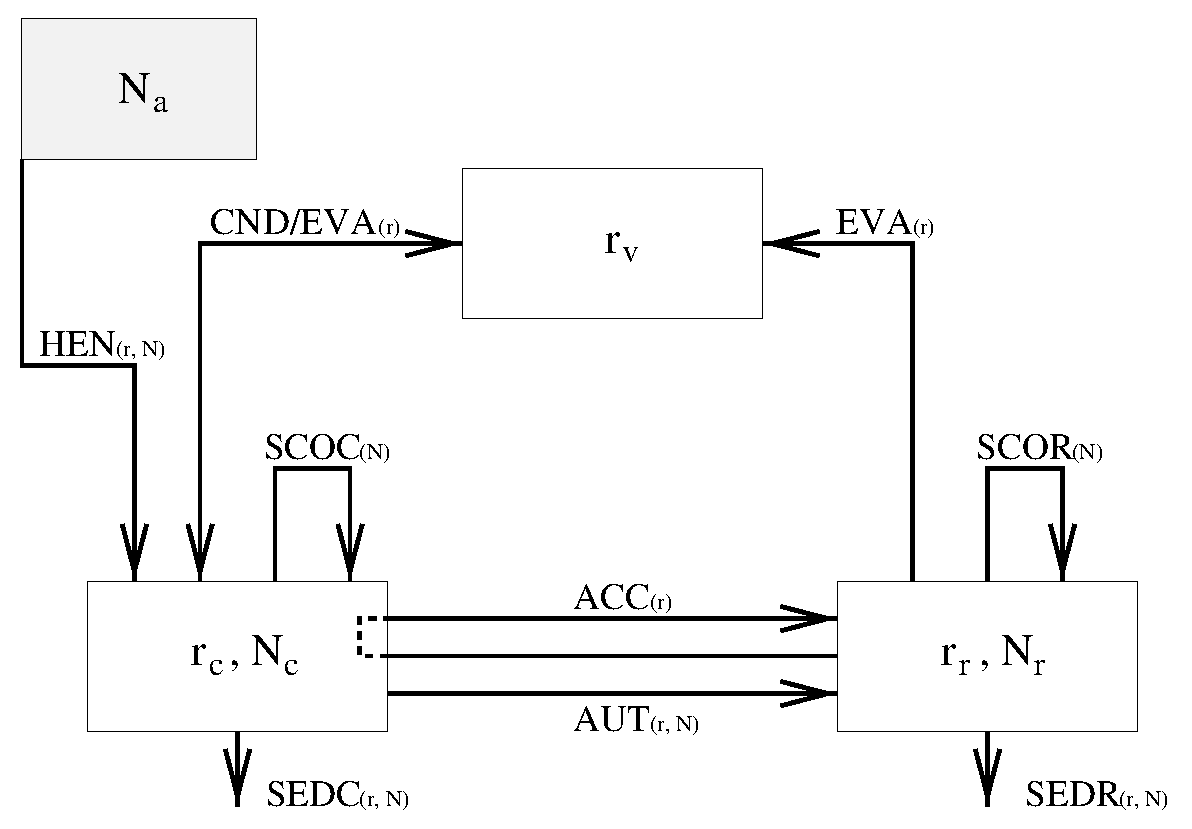
\includegraphics[width=10cm]{\EPSDIR/diagramC2R2.eps}}
\caption{Warm microphysical processes included in the C2R2 scheme (see text for
the acronyms and explanations).}
\label{diagramC2R2fig}
\end{figure}

\begin{table}
\caption{Nomenclature of the microphysical processes involved in (\ref{CONSTN1}a-d).}\label{tabnomen}
\begin{center}
\begin{tabular}{|c|c|c|c|c|}
\hline
%% & & & & \\
Symbols & Mechanisms & Sinks & Sources & Processes \\
\hline \hline
$RVHENC$ & $r_v\ \Longrightarrow \ r_c$ & $r_v$ & $r_c$ & nucleation \\
%% & & & & \\
$CVHENC$ & $N_n\ \Longrightarrow \ N_a$ & $N_n$ & $N_a$ & (implicitly) \\
         & $N_a\ \Longrightarrow \ N_c$ & $N_a$ & $N_c$ & \\
\hline
$RVCONC$ & $r_v\ \Longrightarrow \ r_c$ & $r_v$ & $r_c$ & condensation \\
         & $r_v\ \Longleftarrow \ r_c$ & $r_c$ & $r_v$ & {\&} evaporation \\
\hline
$RCAUTR$ & $r_c+r_c\ \Longrightarrow \ r_r$ & $r_c$ & $r_r$ & autoconversion \\
%% & & & & \\
$CCAUTR$ & $N_c+N_c\ \Longrightarrow \ N_r$ & $N_c$ & $N_r$ & \\
\hline
$RCACCR$ & $r_c+r_r\ \Longrightarrow \ r_r$ & $r_c$ & $r_r$ & accretion \\
%% & & & & \\
$CCACCR$ & $N_c+N_c\ \Longrightarrow \ N_r$ & $N_c$ & $N_r$ & \\
\hline
$RREVAV$ & $r_r\ \Longrightarrow \ r_v$ & $r_r$ & $r_v$ & evaporation \\
\hline
$CRSCOR$ & $N_r+N_r\ \Longrightarrow \ N_r$ & $N_r$ & $N_r$  & self-collection \\ 
%% & & & & break-up \\
$CCSCOC$ & $N_c+N_c\ \Longrightarrow \ N_c$ & $N_c$ & $N_c$  & {\&} break-up \\
\hline
$RSEDR$ & $r_r\ \Longrightarrow \ r_r$ & $r_r$ & $r_r$ & sedimentation \\
%% & & & & \\
$CSEDR$ & $N_r\ \Longrightarrow \ N_r$ & $N_r$ & $N_r$ & \\
\hline
\end{tabular}
\end{center}
\end{table}

\subsubsection{CCN activation (CVHENC) and reversible condensation/evaporation
of droplets (RVCONC)}

The CCN activation  and the condensation growth of cloud droplets are the 
dominant processes affecting distinctly the number concentration ($N_c$) 
and the mixing ratio ($r_c$) of cloud liquid water at the early stage of 
the cloud lifetime. These processes are difficult to model explicitly 
because they depend upon the maximum (CCN activation) and mean (condensation) 
local supersaturation values $s_{v,w}$ in contact with the CCN and the 
droplets. This quantity is not generally well captured in cloud models 
because its scale is highly variable and because the activation process results 
from an unstable thermodynamical equilibrium at short timescales in 
competition with the condensation growth that just tends to absorb any 
excess of supersaturation.

The parameterization of the CCN activation follows the diagnostic and 
integral approach of Twomey (1959) as improved by Cohard et al. (1998) 
where CCN activation spectra are expressed in the following functional 
form:
%
\beq\label{CCNSPEC}
N_{CCN}= C s_{{v,w}}^k F(\mu,\frac{\displaystyle{k}}{\displaystyle{2}},
		  \frac{\displaystyle{k}}{\displaystyle{2}}+1;-\beta s_{{v,w}}^2).
\eeq
%
\noindent $F(a,b,c;x)$ is the hypergeometric function. This form 
adheres more closely to observations of $N_{CCN}$ at large $s_{v,w}$ 
($N_{CCN}$ is finite as $s_{{v,w}}$ goes to infinity) as compared
to the traditional $C s_{{v,w}}^k$ law. Furthermore Cohard et al. (2000c)
show that it is possible to establish parametric relations between the four 
unknowns in (\ref{CCNSPEC}) and characteristics of lognormal distributions
of underlying aerosols with variable chemical composition and solubility.
Thus the $k$, $\beta$ and $\mu$ parameters of
(\ref{CCNSPEC}) can be expressed with the following formulas:
\begin{subequations}\label{SYS2}
\begin{align}
\frac{k}{k_0} & = \Big(\frac{{\rm ln}(\sigma)}{{\rm ln}(\sigma)_0}\Big)^{\alpha_k^{\sigma}},
  \tag{\ref{SYS2}a} \\
\frac{{\beta}}{{\beta}_0} & =
        \Big(\frac{\overline{r}}{\overline{r}_0}\Big)^{\alpha_{\beta}^{\overline{r}}}
    \exp\Big({\raisebox{-0.75ex}{${}^{\alpha_{\beta}^{\sigma}}$}}(\frac{{\rm ln}(\sigma)}{{\rm ln}(\sigma)_0}-1)\Big)
        \Big(\frac{\epsilon_m}{{\epsilon_m}_0}\Big)^{\alpha_{\beta}^{\epsilon_m}}
        \Big(\frac{T}{T_0}\Big)^{\alpha_{\beta}^{T}},
  \tag{\ref{SYS2}b} \\
\frac{{\mu}}{{\mu}_0} & = \Big(\frac{{\rm ln}(\sigma)}{{\rm ln}(\sigma)_0}\Big)^{\alpha_{\mu}^{\sigma}}.
  \tag{\ref{SYS2}c}
\end{align}
\end{subequations}
\addtocounter{equation}{1}
%
\noindent The values of the new coefficients in (\ref{SYS2}a-c) can be taken
from Tables 2 and 3 of Cohard et al. (2000c). The remaining parameter $C$ in
(\ref{CCNSPEC}) is deduced from the total CCN number concentration
($N_{CCN}^{max}$) using
%
\begin{align}
\label{CCNLIM1}
\displaystyle{\lim_{s_{v,w} \rightarrow +\infty}}
N_{CCN}(s_{v,w}) = N_{CCN}^{max} =
  \frac{\displaystyle{C}}{\displaystyle{\beta ^{k/2}}}
   \frac{\displaystyle{\Gamma(k/2 + 1)\Gamma(\mu- k/2)}}
   {\displaystyle{\Gamma(\mu)}}
\end{align}
\addtocounter{equation}{1}
%
\noindent under the condition that $k$ verifies $k<2\mu$ which is always
satisfied here.

Using (\ref{CCNSPEC}) and following Twomey's method, Cohard et al. (1998)
showed that an estimate of the maximum supersaturation $s_{{v,w}_{MAX}}$
is the root of
\beq\label{MAJORS}
s^{k+2}_{{v,w}_{MAX}}F(\mu,\frac{k}{2},\frac{k}{2}+\frac
{3}{2},-\beta s^{2}_{{v,w}_{MAX}})=\frac{\rho_a(\psi_1w)^{3/2}}{2kC\pi\rho_w\psi_2
(G)^{3/2}B(\frac{\displaystyle k}{\displaystyle 2},\frac{\displaystyle 3}
{\displaystyle 2})}.
\eeq
\noindent Substituting values of $s_{v,w}=s_{{v,w}_{MAX}}$ into (\ref{CCNSPEC})
provides an estimate of the potentially activable CCN number concentration, 
so the production rate of newly nucleated droplets is given by comparison 
with CCN that have been already activated. It is also worth to note that
(\ref{CCNSPEC}) and (\ref{MAJORS}) can be easily generalized to a mixture 
of aerosols.

The reversible condensation/evaporation process is treated implicitly 
as a result of a non-iterative vapor saturation adjustment (see Cohard
and Pinty, 2000a).  This treatment is well justified by observations 
that show that the interior of clouds is nearly in thermodynamical equilibrium
($s_{v,w}<1 \%$). The condensation rate is obtained after solving for $T$ 
the equation of the first law of thermodynamics,
\beq\label{THCON}
(T-T^*) + {L_v(T) \over C_{ph}} (r_{vs}(T)-r_v^*) = 0
\eeq
\noindent where $T^*$ and $r_v^*$ are the temperature and vapor mixing 
ratio of an intermediate state after integrating all the other explicit 
processes. $r_{vs}(T)$ is the saturated water vapor mixing ratio, $L_v(T)$ 
the latent heat of vaporization and $C_{ph}$ the heat capacity of cloudy air. 
The condensation rate is given by
\beq\label{RCCON}
RVCONC = max(-r_c, r_v^* - r_{vs}(T))/\delta t
\eeq

\subsubsection{Coalescence}

A short analysis of the stochastic collection equation indicates that bulk 
microphysical schemes always need a 
parameterization for the autoconversion terms (formation of raindrops by droplet
coalescence) while the other processes (including raindrop growth by accretion 
and self-collection) can be treated analytically using the collection kernels 
of Long (1974).

\paragraph{Autoconversion (RCAUTR and CCAUTR)}

The parameterization relies on the work of Berry and Reinhardt (1974) for 
the computation of the RCAUTR term. The parameterization is built on the 
observation that a characteristic water content $L$ of small drops develops 
steadily over a characteristic timescale $\tau$. These two positive 
quantities are expressed in the ranges 20 $\mu$m $\leq D_c \leq$ 36 $\mu$m 
and 0 $\leq \nu_c \leq$ 3 by:
%
\begin{subequations} \label{BERRY}
\begin{align}
L=&2.7 \times 10^{-2}\rho_a r_c
(\dfrac{1}{16}\times 10^{20}\sigma_c^3D_c-0.4) \tag{\ref{BERRY}a}\\
\tau=& 3.7\frac{\displaystyle{1}}{\displaystyle{\rho_a r_c}}
(0.5 \times 10^6\sigma_c-7.5)^{-1} \tag{\ref{BERRY}b}
\end{align}
\end{subequations}
\addtocounter{equation}{1}
%
\noindent where the mean-volume drop diameter $D_c$ and the standard 
deviation $\sigma_c$ are computed using (\ref{MOMENT}). Eqs({\ref{BERRY}a})
and ({\ref{BERRY}b}) are combined to get: 
%
\begin{align}
\label{RCAUT}
RCAUTR = & - max(\frac{\displaystyle{L}}{\displaystyle{\tau}},0.)
\end{align}
%

A suitable parameterization of the CCAUTR rate is more difficult to obtain
because the original Berry and Reinhardt's parameterization tends to 
accumulate the freshly formed drops by autoconversion in the lowest
part of the raindrop spectrum thus preventing the development of sizeable
raindrops. This led Cohard and Pinty (2000a) to the conclusion that it is 
important to restrict the original Berry and Reinhardt formulation:
%
\begin{align}
\label{NCAUT}
CCAUTR = & -3.5 \times 10^9 \;\frac{\displaystyle{\rho_a L}}{\displaystyle{\tau}}
\end{align}
%
\noindent to situations where $D_r<D_h$ where $D_h$ is the "hump diameter"
defined by Berry and Reinhardt (1974). For cases where $D_r>D_h$, it is
assumed that the autoconversion of the cloud droplets does not modify the 
mean-volume diameter so (\ref{NCAUT}) is replaced by:
%
\beq\label{NCCAUTR}
CCAUTR = \frac{\displaystyle{N_r}}{\displaystyle{r_r}} RCAUTR
\eeq
%

\paragraph{Accretion (RCACCR and CCACCR) and self-collections (CCSCOC 
and CRSCOR)}

The processes of accretion and self-collections associated to polynomial 
collection kernels, can be integrated analytically in bulk schemes as 
shown by Cohard and Pinty (2000a). The collection kernels of Long (1974), 
already used by Ziegler (1985), are considered in this study:
%
\beq\label{LONG}
K(D_1,D_2) =
  \begin{cases}
K_2  (D_1^6+D_2^6) & \text{if $D_1\leq 100 \mu$m}, \\
K_1  (D_1^3+D_2^3) & \text{if $D_1 > 100 \mu$m}. \\
  \end{cases}
\eeq
%
\noindent with $K_2=2.59 \times 10^{15}$ m$^{-3}$s$^{-1}$ and 
$K_1=3.03 \times 10^3$ s$^{-1}$. As recommended by Berry and Reinhardt (1974), 
the accretion and the self-collection of raindrops are accounted for once 
$r_r>1.2\times L/\rho_a$. The cumbersome expressions of the different ACC and 
SCO terms have been obtained by Cohard and Pinty (2000a) for the raindrops:
%                                       
\beq\label{ACCR1}
\begin{array}{rl}
{\rm If}\; D_r \geq 100 \mu{\rm m} & \\
CCACCR & = -K_1 N_cN_r                
\Big(\frac{\displaystyle{ \Gamma(\nu_c+3/\alpha_c)}}
{\displaystyle{\Gamma(\nu_c)\lambda_c^3}}+
\frac{\displaystyle{\Gamma(\nu_r+3/\alpha_r)}}
{\displaystyle{\Gamma(\nu_r)\lambda_r^3}}\Big)\\
\\                                      
RCACCR & = -\frac{\displaystyle{\pi}}{\displaystyle{6}}
\frac{\displaystyle{\rho_w}}{\displaystyle{\rho_{a}}} K_1
\frac{ \displaystyle{N_cN_r}}{\displaystyle{\lambda_c^3}}
\Big(\frac{\displaystyle{\Gamma(\nu_c+6/\alpha_c) }}
{\displaystyle{\Gamma(\nu_c)\lambda_c^3}} +
\frac{\displaystyle{\Gamma(\nu_c+3/\alpha_c)}}
{\displaystyle{\Gamma(\nu_c)}}          
\frac{\displaystyle{\Gamma(\nu_r+3/\alpha_r)}}
{\displaystyle{\Gamma(\nu_r)\lambda_r^3}}\Big)\\
\\
CRSCOR & = - K_1 N_r^2 \frac{\displaystyle{\Gamma(\nu_r+3/\alpha_r)}}
                            {\displaystyle{\Gamma(\nu_r)\lambda_r^{3}}}
\end{array}                             
\eeq                                    
%

%
\beq\label{ACCR2}
\begin{array}{rl}
{\rm If}\; D_r < 100 \mu{\rm m} & \\
CCACCR & = -K_2 N_cN_r
\Big(\frac{\displaystyle{ \Gamma(\nu_c+6/\alpha_c)}}
{\displaystyle{\Gamma(\nu_c)\lambda_c^6}}+
\frac{\displaystyle{\Gamma(\nu_r+6/\alpha_r)}}
{\displaystyle{\Gamma(\nu_r)\lambda_r^6}}\Big)\\
\\
RCACCR & = -\frac{\displaystyle{\pi}}{\displaystyle{6}}
\frac{\displaystyle{\rho_w}}{\displaystyle{\rho_{a}}} K_2
\frac{ \displaystyle{N_cN_r}}{\displaystyle{\lambda_c^3}}
\Big(\frac{\displaystyle{\Gamma(\nu_c+9/\alpha_c) }}
{\displaystyle{\Gamma(\nu_c)\lambda_c^6}} +
\frac{\displaystyle{\Gamma(\nu_c+3/\alpha_c)}}
{\displaystyle{\Gamma(\nu_c)}}
\frac{\displaystyle{\Gamma(\nu_r+6/\alpha_r)}}
{\displaystyle{\Gamma(\nu_r)\lambda_r^6}}\Big)\\
\\
CRSCOR & = - K_2 N_r^2 \frac{\displaystyle{\Gamma(\nu_r+6/\alpha_r)}}
                            {\displaystyle{\Gamma(\nu_r)\lambda_r^{6}}}
\end{array}
\eeq
%

and for the cloud droplets
%
\beq\label{SCOC}
\begin{array}{rl}
%{\rm as}\; D_c < 100 \mu{\rm m} & \\
CCSCOC & = - K_1 N_c^2 \frac{\displaystyle{\Gamma(\nu_c+3/\alpha_c)}}
                            {\displaystyle{\Gamma(\nu_c)\lambda_c^{3}}}
\end{array}
\eeq
%

\subsubsection{Break-up}

Break-up is an efficient process acting on the concentration of the large 
drops (a key role to explain the high reflectivity core of the tropical rainband
in the present case study). 

Firstly, collisional break-up is introduced as in Verlinde and 
Cotton (1993), where a bulk collection efficiency $E_c<1$ is used to damp 
the growth of the raindrops by self-collection. In the scheme, the 
preceeding $CRSCOR$ term is multiplied by the $E_c$ factor with the 
following definition:
%
\beq\label{BRUP}
E_c=
  \begin{cases}
1 
  &\text{if $D_r<600 \mu{\rm m}$}, \\
\exp(-2.5 \times 10^{3}(D_r-6 \times 10^{-4}))
  &\text{if $600 \mu{\rm m}\leq D_r<2000 \mu{\rm m}$},\\
0 
  &\text{if $D_r\geq 2000 \mu{\rm m}$}.
  \end{cases}
\eeq
%
\noindent Values of the cutoff diameters in (\ref{BRUP}) have been subjected 
to a specific evaluation in Cohard and Pinty (2000b). 

Secondly and as discussed by Cohard and Pinty (2000b), the inclusion of 
an additional drop size limiter (a substitute for a spontaneous break-up 
parameterization) is necessary to remove the giant drops that can be 
produced spuriously by an unaccurate differential transport of $r_r$ and 
$N_r$ (advection and sedimentation terms). The correction is applied 
whenever $D_r$ is larger than 3000 $\mu$m so beyond the range of active
collisional break-up (see Cohard and Pinty (2000b) for further details).

\subsubsection{Evaporation (RREVAV)}

The evaporation rate of a raindrop population, falling in an undersaturated 
environment ($s_{v,w} \ll 0$) is obtained after performing an analytical 
integration over the whole drop mass spectrum. The size evolution of a single 
evaporating drop of diameter $D$ is given by
%
\beq\label{EVAP1}
   \frac{\displaystyle{d D}}{\displaystyle{d t}} \Big|_{EVA}
 = \frac{\displaystyle{4 s_{v,w} \bar f G}}{\displaystyle{D}}
\eeq
%
\noindent where the ventilation factor $\bar f$, an empirical function of the Reynolds
number $Re=VD/\nu_{cin}$ of the flow, is given by:
%
\beq\label{EVAP2}
\begin{array}{rl}
\bar f &= 0.78 + F Re ^{0.5}
= 0.78 + 0.265\Big[ \Big( \frac{\displaystyle{\rho_{00}}}{\displaystyle{\rho_{a}}} \Big)^{0.4}
                      \frac{\displaystyle{cD^{d+1}}}{\displaystyle{\nu_{cin}}} \Big]^{0.5}\\
\end{array}
\eeq
%
\noindent after inserting (\ref{TERMVEL}). Integrating (\ref{EVAP1}) with (\ref{EVAP2})
and (\ref{GAMMA}) leads to an analytical expression of the evaporation rate that is:
\begin{align}
\label{EVAP3}
RREVAV &= \frac{\displaystyle{1}}{\displaystyle{\rho_{a}}}
\displaystyle{\int_0^{+\infty} 
\frac{\displaystyle{\pi}}{\displaystyle{2}} \rho_w D^2 
\frac{\displaystyle{d D}}{\displaystyle{d t}} \Big|_{EVA} n_r(D) dD }\\
&=\frac{\displaystyle{2 \pi s_{v,w} N_r G}}{\displaystyle{\lambda \Gamma(\lambda)}}
  \frac{\displaystyle{\rho_w}}{\displaystyle{\rho_{a}}}
\Big[ 0.78
+ 0.265 \Big( \frac{\displaystyle{\rho_{00}}}{\displaystyle{\rho_{a}}} \Big)^{0.2} 
    \Big( \frac{\displaystyle{c}}{\displaystyle{\nu_{cin}}}        \Big)^{0.5}
          \frac{\displaystyle{\Gamma (\nu_r+(d+3)/2\alpha_r)}}
	       {\displaystyle{\lambda_r^{(d+1)/2}}} \Big]. \notag
\end{align}
\addtocounter{equation}{1}
Concentrations $N_r$ are not affected by evaporation in the present scheme. 
However if the mean volume drop diameter becomes smaller than 82~$\mu$m 
(the hypothetical size separation between the droplet and drop modes)
then all raindrops are converted into cloud droplets, i.e. $N_c = N_c + N_r; 
r_c = r_c + r_r$ and $N_r = r_r = 0.$ 

\subsubsection{Sedimentation (RSEDR and CSEDR)}

Due to the fact that the terminal velocity of drops depends on their size,
the gravitational sedimentation of hydrometeors is selective if one considers 
the whole range of raindrop spectra. This leads to an efficient size sorting 
phenomenom which is important in the case of warm cumuli where some drops 
can be large enough to fall while smaller ones are delayed and maintained 
in updraft cores for further growth. This differential settling between drops 
is accounted for in two-moment schemes because both sedimentation
fluxes of $N_r$ and $r_r$ are computed:
%\begin{align}
%\label{SEDIM1}
%RSEDR &= \frac{\displaystyle{1}}{\displaystyle{\rho_{a}}}
%\frac{\displaystyle{\partial}}{\displaystyle{\partial z}}
%\displaystyle{\int_0^\infty
%\frac{\pi}{6} \rho_w D^3 V(D) N(D) dD}  \notag \\
%      &= \frac{\displaystyle{1}}{\displaystyle{\rho_{a}}}
%\frac{\displaystyle{\partial}}{\displaystyle{\partial z}}
%\Big[c \big( \frac{\displaystyle{\rho_{00}}}{\displaystyle{\rho_{a}}}\big)
%^{0.4} \rho_{a} r_r
%\frac{\displaystyle{\Gamma(\nu_r+(d+3)/ \alpha_r)}}{\displaystyle{
%\lambda_r^{d}\Gamma(\nu_r+3/ \alpha_r)}}  \Big], \\
%\label{SEDIM2}
%CSEDR &= \frac{\displaystyle{\partial}}{\displaystyle{\partial z}}
%\displaystyle{\int_0^\infty V(D)N(D) dD} \notag \\
%      &= \frac{\displaystyle{\partial}}{\displaystyle{\partial z}}
%\Big[c \big( \frac{\displaystyle{\rho_{00}}}{\displaystyle{\rho_{a}}}\big)
%^{0.4} N_r
%\frac{\displaystyle{\Gamma(\nu_r +d/\alpha_r)}}
%{\displaystyle{\lambda_r^d \Gamma(\nu_r)}}\Big].
%\end{align}
\begin{align}
\label{SEDIM1}
RSEDR &= \frac{\displaystyle{1}}{\displaystyle{\rho_{a}}}
\frac{\displaystyle{\partial}}{\displaystyle{\partial z}}
\displaystyle{\int_0^\infty
\frac{\pi}{6} \rho_w D^3 V(D) n_r(D) dD} \notag \\
      &= \frac{\displaystyle{1}}{\displaystyle{\rho_{a}}}
\frac{\displaystyle{\partial}}{\displaystyle{\partial z}}
\Big[c \big( \frac{\displaystyle{\rho_{00}}}{\displaystyle{\rho_{a}}}\big)
^{0.4} \rho_{a} r_r
\frac{\displaystyle{\Gamma(\nu_r+(d+3)/ \alpha_r)}}{\displaystyle{
\lambda_r^{d}\Gamma(\nu_r+3/ \alpha_r)}}  \Big], \\
\label{SEDIM2}
CSEDR &= \frac{\displaystyle{\partial}}{\displaystyle{\partial z}}
\displaystyle{\int_0^\infty V(D) n_r(D) dD} 
       = \frac{\displaystyle{\partial}}{\displaystyle{\partial z}}
\Big[c \big( \frac{\displaystyle{\rho_{00}}}{\displaystyle{\rho_{a}}}\big)
^{0.4} N_r
\frac{\displaystyle{\Gamma(\nu_r +d/\alpha_r)}}
{\displaystyle{\lambda_r^d \Gamma(\nu_r)}}\Big].
\end{align}
In (\ref{SEDIM1})-(\ref{SEDIM2}), a simple power law dependence in diameter including air
density effect (Foote and Du Toit 1969) has been assumed:
\beq\label{TERMVEL}
V(D)= \Big( \frac{\displaystyle{\rho_{00}}}{\displaystyle{\rho_{a}}}\Big)^{0.4} cD^d,
\eeq


\subsection*{Appendix: List of symbols}
\setlongtables
\begin{longtable}{ll}
$A$&$=4\sigma_{w/a}/R_v T\rho_w$\\
$B(a,b)$&beta function\\
$c$ and $d$&parameters of the fall speed-diameter relationship for the\\
           &water drops\\
$C$&activation spectrum coefficient\\
$C_{vv}$&heat capacity at constant volume of water vapor\\
$C_{pd}$, $C_{pv}$ and $C_{w}$&heat capacity at constant pressure of dry air, water vapor\\
                              &and liquid water\\
$C_{ph}$&$=C_{pd}+r_v C_{pv}+(r_c+r_r)C_{w}$\\
$D$, $D_1$ and $D_2$&drop diameters\\
$D_c$, $D_r$&mean volume drop diameter for cloud droplet and raindrop\\
            &distributions\\
%% $D_{crit}$&critical diameter of newly nucleated droplets\\
$D_v$&diffusivity of water vapor in the air\\
$e_v$&water vapor pressure\\
$e_{vs}$&saturation vapor pressure over water\\
$E_c$&collection efficiency\\
$\bar f$&ventilation factor\\
$F$&ventilation coefficient\\
$F(a,b,c;x)$&hypergeometric function\\
$G(D,T,P)$&$=\displaystyle{{1 \over \rho_w}\Big({R_v T \over e_{vs}(T) D_v} +
{L_v(T) \over k_a T}({L_v(T) \over R_v T} -1)\Big)^{-1}}$\\
$k$ and $k_0$&activation spectrum coefficients\\
$k_a$&heat conductivity of air\\
$K(x,y)$ and $K(D_1,D_2)$&collection kernels\\
$K_1$ and $K_2$&Long's collection kernel coefficients\\
$L$&autoconversion water mass\\
$L_v$&latent heat of vaporization\\
$n$, $n_c$ and $n_r$&total, cloud droplet and raindrop size distributions\\
$N_0$&intercept parameter of an exponential distribution law\\
$N_c$, $N_r$&cloud droplet and raindrop number concentration\\
$N_n$, $N_a$&condensation nuclei and activated CCN number concentration\\
$N_{CCN}$&total activable CCN number concentration\\
$M_w$&molar weight of water\\
$M_i(p)$&$p$\_moment of the $i$\_drop size distribution\\
$P$ and $P_{00}$&pressure and reference pressure (1000 hPa)\\
$\overline{r}$&geometric mean radius of the CCN lognormal distribution\\
$r_v$, $r_c$ and $r_r$&water vapor, cloud water and rain water mixing ratios\\
$r_{vs}$&saturated vapor mixing ratio\\
$R_d$ and $R_v$&gas constant for dry air and water vapor\\
$Re$&Reynolds number\\
$s_{v,w}$&supersaturation ($=e_v/e_{vs}-1$)\\
$s_{{v,w}_{MAX}}$&maximum supersaturation\\
$t$&time\\
$T$ and $T_{00}$&temperature and reference temperature (273.16 K)\\
$V(D)$&drop fall speed of diameter $D$\\
$w$&updraft velocity\\
$x$ and $y$&drop mass\\
$z$&height or vertical coordinate\\
$\alpha_{\{k, \beta, \mu\}}^{\{{\overline r}, {\rm ln}(\sigma), \epsilon_m, T\}}$&adjusted parameters defining the CCN spectrum coefficients\\
$\alpha_c$, $\alpha_r$&dispersion parameter of the generalized gamma distribution\\
                      &law for the cloud droplets and the raindrops\\
$\beta$ and ${\beta}_0$&activation spectrum coefficient\\
$\delta t$&time step\\
$\Gamma(a)$&complete gamma function\\
$\epsilon$&$=R_v/R_d$\\
$\epsilon_m$&aerosol soluble fraction\\
$\theta$&potential temperature\\
$\lambda_c$, $\lambda_r$&slope parameter of the generalized gamma distribution law\\
                        &for the cloud droplets and the raindrops\\
$\mu$ and ${\mu}_0$&activation spectrum coefficients\\
$\nu_c$, $\nu_r$&dispersion parameter of the generalized gamma distribution\\
                &law for the cloud droplets and the raindrops\\
$\nu_{cin}$&kinematic viscosity of air\\
$\Pi$&=$(P/P_{00})^{R_d/C_{pd}}$\\
$\rho_a$ and $\rho_w$&air and liquid water densities\\
$\rho_{00}$&air density at $P=P_{00}$ and $T=T_{00}$\\
$\sigma$&geometric standard deviation of the CCN lognormal distribution\\
$\sigma_c$&standard deviation of cloud droplet distribution\\
$\sigma_{w/a}$&surface tension of water over the air\\
$\tau$&timescale for autoconversion\\
$\psi_1(T,P)$&$=\displaystyle{\frac{g}{TR_d}}\displaystyle{\Big(\frac{L_v}{c_pT}-1
\Big)}$ \\
$\psi_2(T,P)$&$=\displaystyle{\Big(\frac{P}{\epsilon e_{vs}(T)}+
\frac{\epsilon L_v^2} {R_dT^2c_p}} \Big)$\\
\end{longtable}

%
\section{The two-moment microphysical scheme for LES of stratocumulus}\label{KHKO}
\subsection{Introduction}
%

The KHKO scheme is a 2-moment microphysical scheme specially designed for boundary layer clouds. These clouds are low precipitating warm clouds, and not sufficiently thick to produce heavy rain. The precipitating hydrometeors are drizzle only: their diameter are of the order of several dozens of micrometers. The conversion rates that impact drizzle formation and evolution are parameterized according to Khairoutdinov and Kogan (2000) (KK00) microphysical scheme. These processes are autoconversion, accretion, drizzle sedimentation and drizzle evaporation. Microphysical processes that impact cloud formation are parameterized as in the C2R2 scheme: cloud droplet condensation and evaporation follow Langlois (1973) and activation follows Cohard et al. (1998) (see the C2R2 scientific documentation). Moreover cloud droplet sedimentation is resolved by assuming a Stokes flow to calculate the cloud droplets terminal velocity and an analytical distribution to describe the cloud droplet spectra as in the C2R2 scheme.
Microphysical prognostic variables are the same as in the C2R2 scheme: cloud droplet number concentration $N_{c}$ and mixing ratio $r_{c}$, precipitating hydrometeors number concentration $N_{r}$ and mixing ratio $r_{r}$, activated cloud condensation nuclei number concentration $N_{a}$.


The next section describes KK00 (the original scheme of Khairoutdinov and Kogan (2000)) and  KHKO (the corresponding scheme implemented in Meso-NH) specificities and limits.

\subsection{KK00 scheme specifities}


The KK00 scheme is a 2-moment bulk microphysical scheme. All processes are parameterized only as a function of mixing ratios and number concentrations of each category (cloud droplet and drizzle). 
The methodology developed in KK00 consisted to assume firstly a power law relationship between conversion rate and the prognostic variables. Each power law introduces coefficients that have to be determined. These coefficients have been empirically adjusted by using about 100 000 hydrometeors spectra obtained from four 3-D LES simulations of stratocumulus clouds using an explicit (bin) microphysical model. For each of these spectra, autoconversion and accretion conversion rates are calculated by integrating the stochastic collection equation. Then the coefficients in the parameterized expressions are evaluated by regression analysis.

Figure~\ref{figKHKO}a shows the range of cloud droplet mixing ratios and number concentrations of spectra used to evaluate conversion rates. These values are typical of values encountered in stratocumulus as shown in Fig~\ref{figKHKO}b and Fig~\ref{figKHKO}c that represent cloud droplet mixing ratios and number concentrations of spectra measured respectively during the ACE-1 and 
ACE-2 field experiments. The advantage of adjusting coefficients using spectra simulated with an explicit model is that these spectra are representative of boundary layer clouds realistic distributions.

\begin{figure}[!ht]
\centerline{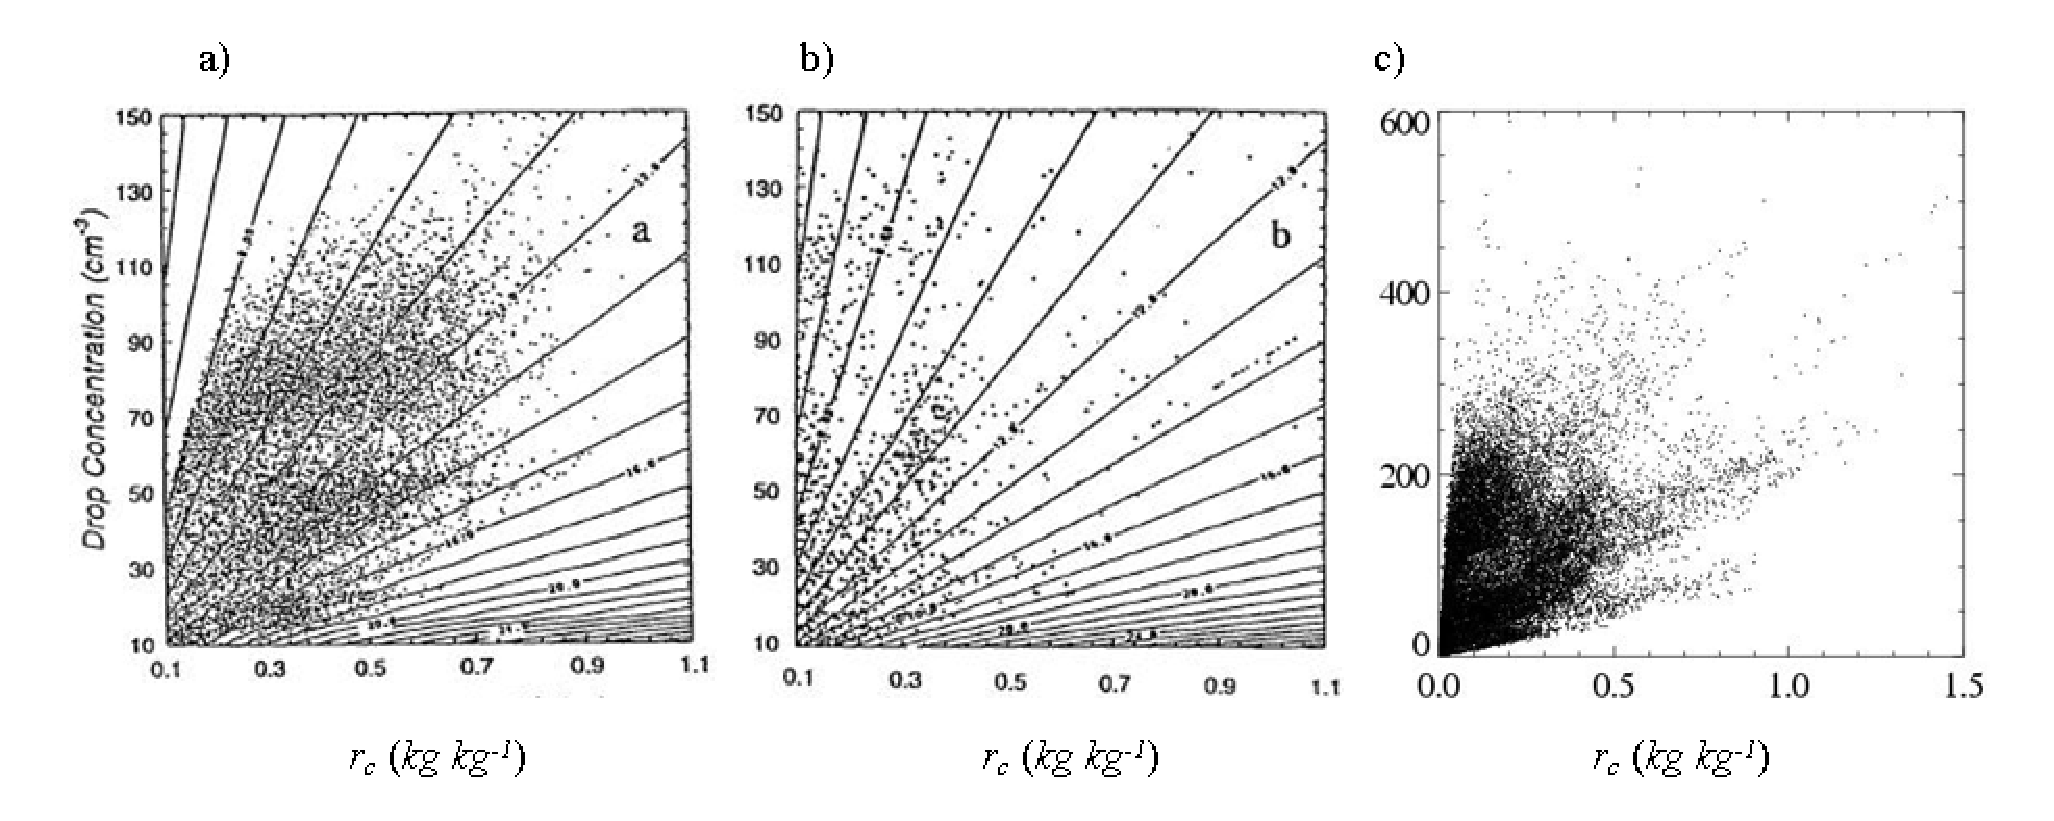
\includegraphics[width=\textwidth]{\EPSDIR/fig_khko1.eps}}
\caption{ a) A scatterplot of the parameter space used to evaluate the coefficients of the KK00  microphysical processes parameterizations. Each data point represents the cloud droplet mixing ratio and the number concentration calculated from an individual hydrometeor size spectrum simulated by the explicit microphysical model.
b) Similar to a) but for the spectra averaged over each aircraft flight leg in stratocumulus cloud during the first phase of ACE-1,
(following Khairoutdinov et Kogan (2000)),
c) Similar to a) but for the ensemble of spectra measured during ACE-2 field experiments (8 flights). Each spectra is averaged with a resolution of about 100~m horizontally. Note that different scales are used for this plot.}
\label{figKHKO} 
\end{figure}


Note that a value for $r_c$ of $1.1$~g~kg$^{-1}$ (the maximum value in Fig.~\ref{figKHKO}a) corresponds to an adiabatic cloud with a depth equal to about 550~m. This value can be calculated by assuming an adiabatic linear relationship between the mixing ratio at cloud top $r_c(H)$ and the cloud depth $H$ with an adiabatic coefficient $C_w$ equal to $2$ $10^{-6}$~kg~m$^{-4}$ : $r_c(H) = C_w H$. This scheme cannot be extended to deep convective clouds. 

In the KK00 scheme, separation between cloud droplets and drizzle is defined at a diameter $D_0$ equal to 50~$\mu$m. This low value permits consideration of drizzle in the precipitating category.

\noindent Parameterizations are expressed as a function of local microphysical values. Thus the scheme is valid only for simulations where microphysical fields are explicitly resolved i.e. in the LES configuration. Resolution must not be more than 200~m horizontally and a few ten of meters vertically (a vertical resolution of 10~m in the cloud is recommended).   


\subsection{System of equations}

For each prognostic variable, conservative equations in KHKO scheme are the following ones:


\begin{subequations} \label{SYSTKHKO}
\begin{align}
\frac{\displaystyle{\partial N_a}}{\displaystyle{\partial t}} =&
\sum \frac{\displaystyle{\partial N_a}}{\displaystyle{\partial t}} \Big|_{NMT}
+ \frac{\displaystyle{\partial N_a}}{\displaystyle{\partial t}} \Big|_{ACT}
+ \frac{\displaystyle{\partial N_a}}{\displaystyle{\partial t}} \Big|_{EVAPC} \tag{\ref{SYSTKHKO}a}\\
\frac{\displaystyle{\partial N_c}}{\displaystyle{\partial t}} =&
\sum \frac{\displaystyle{\partial N_c}}{\displaystyle{\partial t}} \Big|_{NMT}
+ \frac{\displaystyle{\partial N_c}}{\displaystyle{\partial t}} \Big|_{ACT} 
+ \frac{\displaystyle{\partial N_c}}{\displaystyle{\partial t}} \Big|_{SEDC} 
+ \frac{\displaystyle{\partial N_c}}{\displaystyle{\partial t}} \Big|_{AUTO} 
+ \frac{\displaystyle{\partial N_c}}{\displaystyle{\partial t}} \Big|_{ACCR}
+ \frac{\displaystyle{\partial N_c}}{\displaystyle{\partial t}} \Big|_{EVAPC}  \tag{\ref{SYSTKHKO}b}\\
\frac{\displaystyle{\partial r_c}}{\displaystyle{\partial t}} =&
\sum \frac{\displaystyle{\partial r_c}}{\displaystyle{\partial t}} \Big|_{NMT}
+ \frac{\displaystyle{\partial r_c}}{\displaystyle{\partial t}} \Big|_{ACT} 
+ \frac{\displaystyle{\partial r_c}}{\displaystyle{\partial t}} \Big|_{SEDC} 
+ \frac{\displaystyle{\partial r_c}}{\displaystyle{\partial t}} \Big|_{AUTO} 
+ \frac{\displaystyle{\partial r_c}}{\displaystyle{\partial t}} \Big|_{ACCR}
+ \frac{\displaystyle{\partial r_c}}{\displaystyle{\partial t}} \Big|_{CONDC}
+ \frac{\displaystyle{\partial r_c}}{\displaystyle{\partial t}} \Big|_{EVAPC} \tag{\ref{SYSTKHKO}c}\\
\frac{\displaystyle{\partial N_r}}{\displaystyle{\partial t}} =&
\sum \frac{\displaystyle{\partial N_r}}{\displaystyle{\partial t}} \Big|_{NMT}
+ \frac{\displaystyle{\partial N_r}}{\displaystyle{\partial t}} \Big|_{SEDR} 
+ \frac{\displaystyle{\partial N_r}}{\displaystyle{\partial t}} \Big|_{AUTO} 
+ \frac{\displaystyle{\partial N_r}}{\displaystyle{\partial t}} \Big|_{ACCR}
+ \frac{\displaystyle{\partial N_r}}{\displaystyle{\partial t}} \Big|_{EVAPR}   \tag{\ref{SYSTKHKO}d}\\
\frac{\displaystyle{\partial r_r}}{\displaystyle{\partial t}} =&
\sum \frac{\displaystyle{\partial r_r}}{\displaystyle{\partial t}} \Big|_{NMT}
+ \frac{\displaystyle{\partial r_r}}{\displaystyle{\partial t}} \Big|_{SEDR} 
+ \frac{\displaystyle{\partial r_r}}{\displaystyle{\partial t}} \Big|_{AUTO} 
+ \frac{\displaystyle{\partial r_r}}{\displaystyle{\partial t}} \Big|_{EVAPR} \tag{\ref{SYSTKHKO}e}
\end{align}
\end{subequations}
\addtocounter{equation}{1}



\noindent where the subscript $NMT$ refers to Non-Microphysical Tendencies (advection, turbulence, numerics and other physical processes), $ACT$, $SEDC$, $SEDR$, $AUTO$, $ACCR$, $CONDC$, $EVAPC$, $EVAPR$ are the microphysical contributions, i.e. respectively, activation, cloud droplet sedimentation, drizzle sedimentation, autoconversion, accretion, cloud droplet condensation, cloud droplet evaporation and drizzle evaporation. 

\noindent The KK00 scheme does not take into account the drizzle self-collection (on the contrary to C2R2 for raindrops): drizzle diameters are too low for this process to impact the drizzle number concentration $N_r$. Moreover in the KHKO scheme, water vapor condensation on precipitating hydrometeors is not taken into account (as in C2R2).

\noindent In order to close this system of equations the rhs terms are parameterized as a function of the prognostics variables. The next sections describe parameterizations of these processes except for cloud droplet condensation/evaporation and activation, that are identical to the C2R2 scheme. For a description of the latter the reader should refer to the C2R2 documentation.

\subsection{Collection processes}

\paragraph{Autoconversion}

Autoconversion is the process that initializes precipitating hydrometeor spectra. It depends on cloud droplet spectra characteristics. In the KK00 scheme it is assumed to depend on cloud droplets number concentration $N_c$ and mixing ratio $r_c$. After regression analysis on bin model simulations, KK00 obtain the following parameterized expressions for the mixing ratios conversion rates by autoconversion: 

\begin{equation}
\frac{\displaystyle{\partial r_r}}{\displaystyle{\partial t}} \Big|_{AUTO}=1350. r_c^{2.47}N_c^{-1.79}
\label{autoc}
\end{equation}

\begin{equation}
\frac{\displaystyle{\partial r_c}}{\displaystyle{\partial t}} \Big|_{AUTO}=
-\frac{\displaystyle{\partial r_r}}{\displaystyle{\partial t}} \Big|_{AUTO}
\end{equation}


\noindent The cloud droplet number concentration source term is evaluated by assuming that all collected cloud droplet diameters are equal to the mean volume diameter $D_c$:

\begin{equation}
\frac{\displaystyle{\partial N_c}}{\displaystyle{\partial t}} \Big|_{AUTO}=-
\frac{(\frac{\displaystyle{\partial r_r}}{\displaystyle{\partial t}}) \Big|_{AUTO}}
{\frac{\pi\rho_w}{6\rho_a}D_c^3}
\end{equation}


\noindent New drizzle drops are assumed to have the diameter $D_0$ equal to 50~$\mu$m. Thus the drizzle number concentration source term due to autoconversion is:

\begin{equation}
\frac{\displaystyle{\partial N_r}}{\displaystyle{\partial t}} \Big|_{AUTO}=
\frac{\frac{\displaystyle{\partial r_r}}{\displaystyle{\partial t}} \Big|_{AUTO}}
{\frac{\pi\rho_w}{6\rho_a}D_0^{3}}
\end{equation}

\subsubsection{Accretion}

Accretion rate has to be expressed as a function of cloud droplets spectra and precipitating hydrometeors spectra because accretion represents an interaction between the two categories. KK00 assume that accretion rate depends only on cloud droplet and drizzle mixing ratios. After regression analysis the following expressions for mixing ratios conversion rates are obtained: 

\begin{equation}
\frac{\displaystyle{\partial r_r}}{\displaystyle{\partial t}} \Big|_{ACCR}=
67(r_{c}r_{r})^{1.15}
\end{equation}
\begin{equation}
\frac{\displaystyle{\partial r_c}}{\displaystyle{\partial t}} \Big|_{ACCR}=
-\frac{\displaystyle{\partial r_r}}{\displaystyle{\partial t}} \Big|_{ACCR}
\end{equation}

\noindent Similar to autoconversion, cloud droplets number concentration accretion sink term is expressed as the following: 

\begin{equation}
\frac{\displaystyle{\partial N_c}}{\displaystyle{\partial t}} \Big|_{ACCR}=-
\frac{\frac{\displaystyle{\partial r_r}}{\displaystyle{\partial t}} \Big|_{ACCR}}
{\frac{\pi\rho_w}{6\rho_a}D_c^3}
\end{equation}

\noindent Cloud droplets collection by precipitating hydrometeors involves an increase of precipitating hydrometeors mass but not of their number. For that reason there is no accretion source term for the drizzle number concentration.


\subsection{Break-up}

Break-up is applied to achieve a numerical goal only. Drizzle drops are not large enough to take into account this process. However, at some grid point, the drizzle drops number concentration and mixing ratio have non-physical low values that can result in an inconsistency between these two values and thus overly large drizzle mean volume diameters. In order to avoid this divergence, break-up is applied to limit too low values of drizzle number concentration and keep consistency between the drizzle number concentration and mixing ratio.
The same protection is done for the cloud droplets number concentration. The latter is corrected when necessary in order that the cloud droplets mean volume diameter do not exceed the limit diameter between cloud droplets and drizzle i.e. 50~$\mu$m.

\subsection{Drizzle evaporation}

Precipitating drops evaporation rate can be expressed as:
\begin{equation}
\frac{\displaystyle{\partial r_r}}{\displaystyle{\partial t}} \Big|_{EVAPR}=
\frac{2\pi\rho_w}{\rho_a}G(T,P) s_{v,w}\int_{0}^{\infty}Dn_r(D)dD
\end{equation}


\noindent where $G(T,P)$ is a function of temperature and pressure, $n_r(D)$ is the drizzle density function 
and $s_{v,w}$ is the subsaturation ($s_{v,w}=e_v/e_{vs}-1$). 
Note that drizzle drops have a sufficiently low diameter to ignore the ventilation factor. 
By introducing a coefficient $C_{evap}$ equal to the ratio of the drizzle drop mean diameter to the drizzle drop mean volume diameter, it becomes:

\begin{equation}
\frac{\displaystyle{\partial r_r}}{\displaystyle{\partial t}} \Big|_{EVAPR}=
12C_{evap}G(T,P)(\frac{\pi\rho_w}{6\rho_a})^{\frac{2}{3}}r_r^{\frac{1}{3}}N_r^{\frac{2}{3}}s_{v,w}
\end{equation}

\noindent KK00 assume that $C_{evap}$ is a constant parameter. Its value has been adjusted using the spectra derived from the bin model simulations. They propose: $C_{evap}=0.86$. The uncertainty of this parameter is estimated on the order of $15-20\%$.

\noindent KK00 calculate the rate of change of drizzle number concentration as:

\begin{equation}
\frac{\displaystyle{\partial N_r}}{\displaystyle{\partial t}} \Big|_{EVAPR}=
\frac{N_r}{r_r}\frac{\frac{\displaystyle{\partial r_r}}{\displaystyle{\partial t}} \Big|_{EVAPR}}
{\frac{\pi\rho_w}{6\rho_a}D_r^3}
\end{equation}


\noindent Water vapor condensation on drizzle is not taken into account in the model. In the presence of cloud droplets, the amount of water vapor condensed on drizzle is negligible. Because positive supersaturation is encountered in clouds only, it is consistent to neglect condensation on drizzle.


\subsection{Sedimentation} 

\subsubsection{Generalities}

For the two categories of liquid water, number concentration and mixing ratio sedimentation rates  can be expressed respectively as function of the number concentration sedimentation flux $F_{N_i}$ (in m$^{-2}$ s$^{-1}$) and the mixing ratio sedimentation flux $F_{r_i}$ 
(in kg~m$^{-2}$ s$^{-1}$) with $i=[c, r]$.

\begin{equation}
\frac{\displaystyle{\partial N_i}}{\displaystyle{\partial t}} \Big|_{SED_i}=
\frac{\displaystyle{\partial F_{N_i}}}{\displaystyle{\partial z}}
\end{equation}

\begin{equation}
\frac{\displaystyle{\partial r_i}}{\displaystyle{\partial t}} \Big|_{SED_i}=
\frac{1}{\rho_a}\frac{\displaystyle{\partial F_{r_i}}}{\displaystyle{\partial z}}
\end{equation}

\noindent with : $F_{N_i}=V_{N_i}N_i$ and $F_{r_i}=V_{r_i}\rho_ar_i$,

\noindent and : 

\begin{equation}
V_{N_i}=\frac{F_{N_i}}{N_i}=\frac{\int_{0}^{\infty}v(D)n_i(D)dD}{\int_{0}^{\infty}n_i(D)dD}
\end{equation}

\begin{equation}
V_{r_i}=\frac{F_{r_i}}{\rho_ar_i}=\frac{\int_{0}^{\infty}\frac{\pi}{6}\rho_wD^3v(D)n_i(D)dD}{\int_{0}^{\infty}\frac{\pi}{6}\rho_wD^3n_i(D)dD}
\end{equation}


\noindent $V_{r_i}$ is an average weighted by the third momentum of the distribution. 
For a non-monodispersed distribution, the mean terminal velocity of the mixing ratio $V_{r_i}$ is different and greater than the mean terminal velocity of the hydrometeors $V_{N_i}$, because the flux of the hydrometeor mixing ratio is driven by hydrometeors of larger diameter.

\subsubsection{Drizzle sedimentation}

KK00 propose parameterized expressions of the velocity of the drizzle number concentration and the velocity of the mixing ratio as a function of the drizzle distribution mean volume diameter $D_r$:

\begin{equation}
V_{N_r}=0.0035D_r-0.1
\end{equation}
 
\begin{equation}
V_{r_r}=0.006D_r-0.2
\end{equation}


\noindent The coefficients have been tuned against the spectra simulated with the explicit model.

\subsubsection{Cloud droplets sedimentation}

KHKO introduces cloud droplet sedimentation on the contrary to 
KK00 parameterization, because this process has an impact on cloud evolution by reducing entrainment at cloud top (Ackerman et al. 2004; Bretherton et al. 2007). As in the C2R2 scheme, it is parameterized by assuming a Stokes law to calculate the cloud droplets terminal velocity and by assuming an analytical distribution to represent cloud droplet spectra. The analytical distribution used is a generalized gamma law (cf. C2R2 documentation). This law can be expressed as a function of $r_c$ and $N_c$ and two free parameters $\alpha_c$ and $\nu_c$. 

After integration, the sedimentation fluxes for the cloud droplet number concentration and the mixing ratio respectively are the following:

\begin{equation}
F_{N_c}=k_1N_cD_c^2\frac{\Gamma(\nu_c+\frac{2}{\alpha_c})}{\Gamma(\nu_c+\frac{3}{\alpha_c})^{\frac{2}{3}}}\Gamma(\nu_c)^{-\frac{1}{3}}
\end{equation}

\begin{equation}
F_{r_c}=k_2N_cD_c^5\frac{\Gamma(\nu_c+\frac{5}{\alpha_c})}{\Gamma(\nu_c+\frac{3}{\alpha_c})^{\frac{5}{3}}}\Gamma(\nu_c)^{\frac{2}{3}}
\end{equation}

\noindent where $\Gamma(x)$ is the gamma function and $\alpha_c=3$, $\nu_c=2$. These values have been adjusted by comparison with measured cloud droplet spectra during ACE-2 field campaign (Geoffroy 2007).




\subsection*{Appendix: List of symbols}
\setlongtables
\begin{longtable}{ll}

$C_{evap}$ &ratio of the drizzle drop mean radius \\
           &to the drizzle drop mean volume radius\\
$D_0$&separation between cloud droplets and drizzle (=$50$ $\mu$m)\\
$D_c$, $D_r$&mean volume drop diameter for cloud droplet and drizzle\\
            &distributions\\
$D_v$&diffusivity of water vapor in the air\\
$e_v$&water vapor pressure\\
$e_{vs}$&saturation vapor pressure over water\\
$F_{N_c}, F_{r_c}$&cloud number concentration and mixing ratio sedimentation flux\\
$F_{N_r}, F_{r_r}$&drizzle number concentration and mixing ratio sedimentation flux\\
$G(T,P)$&= $ =\frac{1}{\rho_w}(\frac{R_vT}{e_{vs}(T)D_v}+\frac{L_v(T)}{k_aT}(\frac{L_v(T)}{R_vT}-1))^{-1}$ \\
$k_a$&heat conductivity of air\\
$L_v$&latent heat of vaporisation\\
$n$, $n_c$ and $n_r$&total, cloud droplet and drizzle size distributions\\
$N_c$, $N_r$&cloud droplet and drizzle number concentration\\ 
$N_a$ &activated CCN number concentration\\
$P$ &pressure\\

$r_v$, $r_c$ and $r_r$&water vapor, cloud droplets and drizzle mixing ratios\\
$r_{vs}$&saturated water vapor mixing ratio\\
$R_v$&gaz constant for water vapor\\
$s_{v,w}$&supersaturation ($=e_v/e_{vs}-1$)\\
$T$&temperature\\
$v(D)$&Hydrometeor of diameter $D$ terminal velocity \\
$V_{N_r}, V_{r_r}$&drizzle number concentration and mixing ratio mean terminal velocity\\
$\alpha_c$, $\nu_c$&dispersion parameters of the generalized gamma distribution\\
                      &law for the cloud droplets distribution\\
$\rho_a$ and $\rho_w$&air and liquid water densities\\
$\Gamma(a)$&complete gamma function\\
\end{longtable}


\section{References}
\parindent 0truecm
\por
Berry, E. X., and R. L. Reinhardt, 1974: An analysis of cloud drop growth by
        collection: Part II. single initial distributions.
        {\it J. Atmos. Sci.},
        {\bf 31},
        1825-1831.
\por
Bretherton, C. S., P. N. Blossey, and J. Uchida, 2007: Cloud droplet sedimentation, entrainment efficiency,
           and subtropical stratocumulus albedo.
           {\it Geophys. Res. Lett.},
           {\bf 34,} 
           L03813
\por
Cohard, J.-M., J.-P. Pinty, and C. Bedos, 1998: Extending Twomey's analytical
        estimate of nucleated cloud droplet concentrations from CCN spectra.
        {\it J. Atmos. Sci.},
        {\bf 55,}
        3348-3357.
\por
Cohard, J.-M., and J.-P. Pinty, 2000a: A comprehensive two-moment warm
        microphysical bulk scheme. Part I: Description and selective tests.
        {\it Q. J. R. Meteorol. Soc.},
        {\bf 126},
        1815-1842.
\por
Cohard, J.-M., and J.-P. Pinty, 2000b: A comprehensive two-moment warm
        microphysical bulk scheme. Part I: 2D experiments with a
        non-hydrostatic model.
        {\it Q. J. R. Meteorol. Soc.},
        {\bf 126},
        1843-1859.
\por
Cohard, J.-M., J.-P. Pinty, and K. Suhre, 2000c: On the parameterization of
        activation spectra from CCN microphysical properties.
        {\it J. Geophys.  Res.},
        {\bf 105},
        D9,
        11753-11766.
\por
Foote, G. B., and P. S. Du Toit, 1969: Terminal velocity of raindrops aloft.
{\it J. Appl. Meteor.}, {\bf 8}, 249-253.
\por
Geleyn, J.-F., B. Catry, Y. Bouteloup, and R. Brozkova, 2008. A statistical approach for 
        sedimentation inside a micro-physical precipitation scheme.
        {\it Tellus},
        {\bf 60A},
        649-662.
\por
Geoffroy, O., 2007: Modelisation LES des precipitations dans les nuages de couche limite et parametrisation pour les GCM, Ph.D. thesis, Universite Paul Sabatier (Toulouse III).
\por
Kessler, E., 1969: On the distribution and continuity of water sustance in
atmospheric circulations. {\it Meteor. Monog.}, {\bf 10}, N$^\circ$ 32, 84pp.
\por
Khairoudinov, M., and Y. Kogan, 2000: A new cloud physics parameterization
        in a large-eddy simulation model of marine stratocumulus.
        {\it Mon. Wea. Rev.},
        {\bf 128,}
        229-243.
\por
Langlois, W.E., 1973: A rapidly convergent procedure for computing large-scale
condensation in a dynamical weather model. {\it Tellus}, {\bf 25}, 86-87.
\por
Long, A. B., 1974: Solutions to the droplet collection equation for polynomial
        kernels.
        {\it J. Atmos. Sci.},
        {\bf 31},
        1040-1057.
\por
Liu, J. Y, and H. D. Orville, 1969: Numerical modeling of precipitation and cloud
shadow effects on mountain-induced cumuli. {\it J. Atmos. Sci.}, {\bf 26},
1283-1298.
\por
Press, W. H., S. A. Teukolsky, W. T. Vetterling, and B. P. Flannery, 1992:
        {\it Numerical Recipes in FORTRAN: The Art of Scientific Computing.}
        2nd Ed.
        Cambridge University Press,
        963 pp.
\por
Pruppacher, H. R and J. D. Klett, 1978: Microphysics of clouds and precipitation.
Reidel, 714pp
\por
Rood, R. B., 1987: Numerical advection algorithms and their role in atmospheric
transport and chemistry models. {\it Review of Geoph.}, {\bf 25}, 71-100.
\por
Twomey, S., 1959: The nuclei of natural cloud formation. Part II: The
        supersaturation in natural clouds and the variation of cloud droplet
        concentration.
        {\it Geophys. Pure Appl.},
        {\bf 43},
        243-249.
\por
Verlinde, J, P. J. Flatau, and W. R. Cotton, 1990:
        Analytical solution to the collection growth equation: comparison with
        approximate methods and application to cloud microphysics
        parameterization schemes.
        {\it J. Atmos. Sci.},
        {\bf 47},
        2871-2880.
%%%%%%%%%%%%%%%%%%%%%%%%%%%%%%%%%%%%%%%%%%%%%%%%%%%%%%%%%%%%%%%%%%%%%%%%%%%%%%
%%%%%%%%%%%%%%%%%%%%%%%%%%%%%%%%%%%%%%%%%%%%%%%%%%%%%%%%%%%%%%%%%%%%%%%%%%%%%%
%%%%%%%%%%%%%%%%%%%%%%%%  END OF WARM MICROPHYSICS %%%%%%%%%%%%%%%%%%%%%%%%%%%
%%%%%%%%%%%%%%%%%%%%%%%%%%%%%%%%%%%%%%%%%%%%%%%%%%%%%%%%%%%%%%%%%%%%%%%%%%%%%%
%%%%%%%%%%%%%%%%%%%%%%%%%%%%%%%%%%%%%%%%%%%%%%%%%%%%%%%%%%%%%%%%%%%%%%%%%%%%%%
